
In this section, we present a complete $\des$-Wilf equivalence classification for quasi-consecutive patterns of length four. As a motivational background, we comment briefly on the Wilf equivalence classification for quasi-consecutive patterns of length four. In total there are $4!=24$ patterns. Upon taking complement, only half of them need to be considered. It was already conceived by Baxter and Pudwell \cite[Table 6]{BP12} that these twelve patterns split into five Wilf equivalent classes. Their enumeration sequences have all been registered on the OEIS (see the last column in Table~\ref{tab: classifications of length 4}). Many of these equivalences could be easily deduced from Theorem~\ref{thm:eli-kit}, with the remaining ones conjectured in \cite[Conj.~17]{BP12} and later confirmed by Baxter and Shattuck~\cite{BS15}. In fact, almost all length four vincular patterns (not only the quasi-consecutive ones) have been classified according to the Wilf equivalence, with two pairs
$$\underline{23}14\sim 1\underline{23}4,\text{ and } \underline{14}23\sim 2\underline{14}3$$
raised as a conjecture in \cite{BS15}. Solving them would then complete the Wilf equivalence classification for all length four vincular patterns.

When we take the descent number into consideration, numerical data (see Table~\ref{tab: descent vector of length 4}) seems to suggest that there are fourteen different classes of quasi-consecutive patterns. The \textit{descent vector} of pattern $\omega$ at level $n$ is defined as $(a_{n,0}^{\omega},a_{n,1}^{\omega},\ldots,a_{n,n-1}^{\omega})$
where $a_{n,k}^{\omega}=|\{\pi\in \S_n(\omega):\des(\pi)=k\}|$. The different descent vectors shown in the third column of Table~\ref{tab: descent vector of length 4} make it evident that there should be at least fourteen distinctive classes. To show that there are indeed fourteen classes, we are going to construct descent preserving bijections for the patterns contained in the same class, ranging from class No.~1 to class No.~6. For the singleton patterns $\underline{123}4$ and $\underline{321}4$, we apply the generalized run theorem (see Theorem~\ref{thm:gen run thm}) to compute their generating functions in the next section. All these results are summarized in Table~\ref{tab: classifications of length 4}. Also note that due to Proposition~\ref{omega--omega^c}, only half of the patterns need to be considered (one out of each complementary pair). So for instance, we shall construct a bijection between $\S_n(\underline{134}2)$ and $\S_n(\underline{124}3)$ to explain the $\des$-Wilf equivalence between these two patterns in class No.~5, but omit the result for the two patterns in class No.~6 since $\underline{431}2=(\underline{124}3)^c$ and $\underline{421}3=(\underline{134}2)^c$. This also explains why we only include seven classes in Table~\ref{tab: classifications of length 4}.

\begin{table}[h!]
    \setlength{\tabcolsep}{15pt}%调整列宽
    \renewcommand{\arraystretch}{1.2}%调整行距
    \begin{center}
      \begin{tabular}{c|c|c} 
        Class No. & Pattern $\sigma j$ & Descent vector of $\sigma j$ for $n=7$ \\
        \hline
        1 & \underline{312}4,\ \underline{231}4,\ \underline{241}3  & 1,\ 78,\ 724,\ 1706,\ 1041,\ 120,\ 1 \\
        2 & \underline{213}4,\ \underline{132}4,\ \underline{142}3  & 1,\ 110,\ 894,\ 1648,\ 897,\ 120,\ 1 \\
        3 & \underline{243}1,\ \underline{324}1,\ \underline{314}2  & 1,\ 120,\ 1041,\ 1706,\ 724,\ 78,\ 1 \\
        4 & \underline{342}1,\ \underline{423}1,\ \underline{413}2  & 1,\ 120,\ 897,\ 1648,\ 894,\ 110,\ 1 \\
        5 & \underline{134}2,\ \underline{124}3  & 1,\ 56,\ 637,\ 1756,\ 1089,\ 120,\ 1 \\
        6 & \underline{431}2,\ \underline{421}3  & 1,\ 120,\ 1089,\ 1756,\ 637,\ 56,\ 1 \\ 
        7 & $\underline{123}4$ & 0,\ 0,\ 481,\ 2022,\ 1191,\ 120,\ 1  \\ 
        8 & $\underline{321}4$ & 1,\ 120,\ 1119,\ 1853,\ 665,\ 56,\ 1   \\
        9 & $\underline{214}3$ & 1,\ 120,\ 1080,\ 1740,\ 639,\ 56,\ 1   \\ 
        10 & $\underline{412}3$ & 1,\ 56,\ 632,\ 1732,\ 1080,\ 120,\ 1   \\
        11 & $\underline{143}2$ & 1,\ 120,\ 1080,\ 1732,\ 632,\ 56,\ 1   \\ 
        12 & $\underline{341}2$ & 1,\ 56,\ 639,\ 1740,\ 1080,\ 120,\ 1   \\ 
        13 & $\underline{234}1$ & 1,\ 56,\ 665,\ 1853,\ 1119,\ 120,\ 1   \\
        14 & $\underline{432}1$ & 1,\ 120,\ 1191,\ 2022,\ 481,\ 0,\ 0   
      \end{tabular}
    \end{center}
  \caption{Fourteen $\des$-Wilf equivalence classes with their descent vectors for $n=7$}
  \label{tab: descent vector of length 4}
\end{table}

For certain given patterns $\alpha$ and $\beta$, we divide $\S_n$ into four disjoint subsets:
\begin{align*}
  \S_n(\alpha,\beta)&:=\S_n(\alpha) \bigcap \S_n(\beta), \\
  \S_n(\alpha,\check{\beta})&:=\{\pi \in \S_n(\alpha): \beta\text{ occurs in }\pi\} ,\\
  \S_n(\check{\alpha},\beta)&:=\{\pi \in \S_n(\beta): \alpha\text{ occurs in }\pi\} ,\\
  \S_n(\check{\alpha},\check{\beta})&:=\{\pi \in \S_n:\text{both }\alpha\text{ and }\beta\text{ occur in }\pi\} . 
\end{align*}

When constructing a bijection between, say $\S_n(\alpha)$ and $\S_n(\beta)$, we usually set the permutations in $\S_n(\alpha,\beta)$ to be fixed points, and try to find a $\des$-preserving bijection between $\S_n(\alpha,\check{\beta})$ and $\S_n(\check{\alpha},\beta)$, then $\alpha \overset{\des}{\sim }\beta$ follows immediately.

We note that a bijective proof of $\underline{312}4 \overset{\des}{\sim }\underline{231}4\overset{\des}{\sim }\underline{241}3$ has already appeared in \cite{BDGZ19}. It was proved via bijections constructed on the complement sets of pattern avoiding permutations. Their proof of $\underline{312}4 \overset{\des}{\sim }\underline{231}4$ goes roughly as follows: if $\pi \in \S_n(\widecheck{\underline{312}4},\widecheck{\underline{231}4})$,
then $\pi$ is a fixed point; otherwise they find a special occurrence of pattern $\underline{312}4$ in $\pi$, change it to an occurrence of $\underline{231}4$, claiming that this results in a bijection from $\S_n(\widecheck{\underline{312}4},\underline{231}4)$ to $\S_n(\underline{312}4,\widecheck{\underline{231}4})$. But they overlooked the case when there are two or more occurrences of pattern $\underline{312}4$ in $\pi$. In that case, via the bijection, say $\phi$ in \cite{BDGZ19}, $\phi(\pi)$ actually falls in $\S_n(\widecheck{\underline{312}4},\widecheck{\underline{231}4})$. Hence the above proof found in \cite{BDGZ19} is flawed. Their proof of $\underline{231}4\overset{\des}{\sim }\underline{241}3$ is incorrect for the same reason. Moreover, it is worth noting that the Wilf equivalences $\underline{231}4\sim\underline{241}3$, $\underline{132}4\sim\underline{142}3$, and $\underline{134}2\sim\underline{124}3$ are covered by Baxter and Shattuck's general equivalence results in \cite[Thm.~6 and Thm.~9]{BS15}, and it was remarked there that their proof actually shows the stronger $\des$-Wilf equivalences. Nevertheless, comparing to their inductive approach, our bijective proofs below are described via certain algorithms and seem to be more explicit.

Before we get into the bijective proofs, we would like to point out that $\underline{312} \overset{\des}{\sim }\underline{231} $ by Proposition~\ref{omega--omega^rc}, then we can apply Corollary~\ref{col:structure} to deduce that $\underline{312}4 \overset{\des}{\sim }\underline{231}4$. A similar argument leads to $\underline{213}4 \overset{\des}{\sim }\underline{132}4$. Alternatively, we present the following bijective approach. 

\begin{table}[h!]
\setlength{\tabcolsep}{9pt}  %调整列宽
\renewcommand{\arraystretch}{1.2}  %调整行距
 \begin{center}
 \begin{tabular}{c|c|c|c} 
 Pattern $\sigma j$ & Bijections & $A^{\sigma}(x,t)$ & OEIS entry\\ \hline
 \underline{312}4,\ \underline{231}4,\ \underline{241}3 & Theorems~\ref{312-4--231-4} and \ref{231-4--241-3} & Corollary~\ref{231} & A071075 \\
 \underline{213}4,\ \underline{132}4,\ \underline{142}3 & Theorems~\ref{213-4--132-4} and \ref{132-4--142-3} & Proposition~\ref{132} & A071075\\
 \underline{134}2,\ \underline{124}3 & Theorem~\ref{134-2--124-3} & ? & A200403 \\
 $\underline{123}4$ & N/A & \eqref{Sn(123)des} & A071076 \\ 
 $\underline{321}4$ & N/A & \eqref{Sn321des} & A071076 \\
 $\underline{214}3$ & N/A & ? & A200405 \\ 
 $\underline{412}3$ & N/A & ? & A200404
 \end{tabular}
 \end{center}
 \caption{Classifications of $\sigma j$ of length $4$}
 \label{tab: classifications of length 4}
\end{table}

\begin{theorem}\label{312-4--231-4}
  We have the $\des$-Wilf equivalence $\underline{312}4 \overset{\des}{\sim }\underline{231}4$. 
\end{theorem}

\begin{proof}
  It suffices to construct a $\des$-preserving bijection 
  $$f: \S_n(\widecheck{\underline{312}4},\underline{231}4) \to \S_n(\underline{312}4,\widecheck{\underline{231}4}).$$
  Suppose $\pi\in \S_n(\widecheck{\underline{312}4},\underline{231}4)$. 
  We first find all occurrences of $\underline{312}4$ in $\pi$, and
  let $A^{\pi}$ be the set of the elements playing the role of $``4"$ in all occurrences of $\underline{312}4$ in $\pi$. Select the largest element in $A^{\pi}$, say $\pi_{j_1}$ for a certain $j_1$.
  Next find all occurrences of $\underline{312}4$ in $\pi^1:=\pi_{j_1+1} \pi_{j_1+2}\cdots \pi_n$ if any. Let $A^{\pi^1}$ be the set of the elements contained in $\pi^1$ playing the role of $``4"$ in any occurrence of $\underline{312}4$ in $\pi^1$, select the largest element in $A^{\pi^1}$, say $\pi_{j_2}$ for a certain $j_2$. Keep doing this until we arrive at a certain $\pi_{j_l}$ so that the suffix $\pi_{j_l+1}\pi_{j_l+2}\cdots \pi_{n}$ is $\underline{312}4$-avoiding. It follows that $\pi_{j_1}>\pi_{j_2}>\cdots>\pi_{j_l}$ and $j_1<j_2<\cdots<j_l$.
  For instance, if $\pi=867953124$, then $\pi_4=9$ and $\pi_9=4$ would be selected with $j_1=4$ and $j_2=9$.

  Next for all $k,\; 1\le k\le l$, we find $\pi_{i_k}$, which is the rightmost element to the left of $\pi_{j_k}$ such that $\pi_{i_k}>\pi_{j_k}$. For $1<k\le l$, such a $\pi_{i_k}$ always exists since at least we have $\pi_{j_{k-1}}>\pi_{j_k}$. If such a $\pi_{i_1}$ does not exist, then we set $i_1=0$ and $\pi_0=\infty$. This happens when $\pi_{j_1}$ is a left-to-right maximum. 
  % In what follows, we assume that $\pi_{i_1}$ exists. 
  Figure~\ref{fig:312-4} illustrates the relations of elements in $\pi$. 
  \begin{figure}[ht]
    \centering
    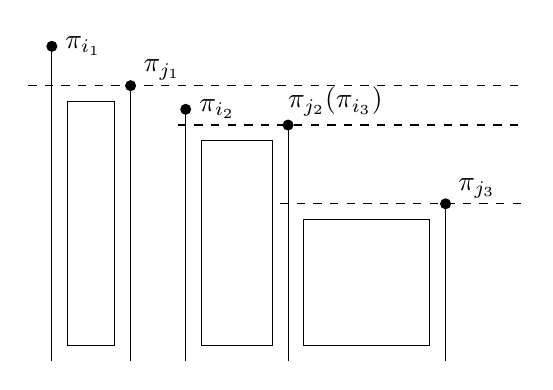
\begin{tikzpicture}
      \draw (0,0)--(0,4);
      \fill (0,4) circle[radius=2pt];
      \node at (0.4,4) {$\pi_{i_1}$};
      \draw (1,0)--(1,3.5);
      \fill (1,3.5) circle[radius=2pt];
      \node at (1.4,3.7) {$\pi_{j_1}$};
      \draw[dashed] (-0.3,3.5) -- (6,3.5);
      \draw (0.2,3.3) rectangle (0.8,0.2);

      \draw (1.7,0)--(1.7,3.2);
      \fill (1.7,3.2) circle[radius=2pt];
      \node at (2.1,3.2) {$\pi_{i_2}$};
      \draw (3,0)--(3,3);
      \fill (3,3) circle[radius=2pt];
      \node at (3.6,3.3) {$\pi_{j_2}(\pi_{i_3})$};
      \draw[dashed] (1.6,3) -- (6,3);
      \draw (1.9,2.8) rectangle (2.8,0.2);

      \draw (5,0)--(5,2);
      \fill (5,2) circle[radius=2pt];
      \node at (5.4,2.2) {$\pi_{j_3}$};
      \draw[dashed] (2.9,2) -- (6,2);
      \draw (3.2,1.8) rectangle (4.8,0.2);
    \end{tikzpicture}
    \caption{An illustration of choosing $\pi_{j_k}$ and $\pi_{i_k}$, $1\le k\le l$}
    \label{fig:312-4}
  \end{figure}

  The choices of $\pi_{i_k},\pi_{j_k}(1\le k \le l)$ imply that,  
  for all $1\le k \le l$, 
  \begin{enumerate}[label=(\roman*)]
      \item there is no $\underline{231}4$ pattern in $\pi_1\pi_2\cdots \pi_{n}$;
      \item $\pi_{i_k+1},\pi_{i_k+2},\cdots ,\pi_{j_k-1}<\pi_{j_k}<\pi_{i_k}$;
      \item there is no $\underline{312}4$ pattern in $\pi_{j_{k-1}+1}\pi_{j_{k-1}+2}\cdots \pi_{i_{k}}(j_{0}:=0)$;
      \item there must be a $\underline{312}4$ pattern in $\pi_{i_k+1} \pi_{i_k+2}\cdots \pi_{j_k}$;
      \item $j_k-i_k\ge 4$.
  \end{enumerate}
  Now we obtain the image permutation $f(\pi)$ from $\pi$ by keeping the positions and values of both $\pi_{i_k}$ and $\pi_{j_k}$, while transforming the subword $\pi_{i_k+1}\pi_{i_k+2}\cdots \pi_{j_{k}-1}$ to $\pi'_{i_k+1}\pi'_{i_k+2}\cdots \pi'_{j_k-1}$, for all $1\le k\le l$, where
  $\pi'_{i_k+1}\pi'_{i_k+2}\cdots \pi'_{j_k-1}$ is the permutation on
  $\{\pi_{i_k+1},\pi_{i_k+2},\cdots, \pi_{j_k-1}\}$ such that
  $$\std(\pi'_{i_k+1}\pi'_{i_k+2}\cdots \pi'_{j_k-1})=(\std (\pi_{i_k+1}\pi_{i_k+2}\cdots \pi_{j_k-1}))^{rc}.$$
  For instance, $f(867953124)=786952314$. Moreover, one should be able to verify the following facts for all $1\le k \le l$.
  \begin{enumerate}[label=(\roman*)]
      \item $\des(\pi)=\des(f(\pi))$ since $\pi_{i_k}$ and $\pi_{j_k}$ are greater than 
      the elements in \\ $\{\pi_{i_k+1},\pi_{i_k+2},\cdots, \pi_{j_k-1}\}$, and the composition $\phi_r\circ\phi_c$ preserves the descent number.
      \item all occurrences of $\underline{312}4$ in $\pi_{i_k+1} \pi_{i_k+2}\cdots \pi_{j_k}$ become occurrences of $\underline{231}4$ in $\pi_{i_k+1}' \pi_{i_k+2}'\cdots \pi_{j_k}'$.
      \item there is no $\underline{312}4$ pattern in $f(\pi)$.
      \item $\pi_{j_k}=f(\pi)_{j_k}$ is also the largest element of $B^{f(\pi)^{k-1}}$, where
      $B^{f(\pi)^{k-1}}$ is        
      the set of elements playing $``4"$ in each occurrence of $\underline{231}4$ in
      $$f(\pi)_{j_{k-1}+1}f(\pi)_{j_{k-1}+2}\cdots f(\pi)_{i_k} f(\pi)_{i_k+1}\cdots f(\pi)_{j_k-1} f(\pi)_{j_k}\cdots f(\pi)_n,\quad (f(\pi)^0:=f(\pi)).
      $$
      Moreover, $A^{\pi^k}=B^{f(\pi)^{k}}$ for all $0\le k \le l-1$ $(\pi^0=\pi,f(\pi)^{0}=f(\pi))$.
      \item there is no $\underline{231}4$ pattern in $\pi_{j_{k-1}+1}\pi_{j_{k-1}+2}\cdots \pi_{i_{k}}$.
  \end{enumerate}
  Therefore, $f(\pi)\in \S_n(\underline{312}4,\widecheck{\underline{231}4})$.

  To show that $f$ is invertible, the key thing to notice is that $f$ keeps the ``maximality" of $\pi_{j_k}(1\le k \le l)$. The inverse mapping $f^{-1}$ is constructed similarly as $f$, except now finding $\pi_{j_k}$ and $\pi_{i_k}$ is with respect to the pattern $\underline{231}4$,
  and we implement the same transformation on the subword $\pi_{i_k+1}\pi_{i_k+2}\cdots \pi_{j_{k}-1}$.
\end{proof}

\begin{remark}
  The bijection $f$ constructed in Theorem~\ref{312-4--231-4} also preserves the statistic $\inv $,
  i.e., $\inv (\pi)=\inv (f(\pi))$ for $\pi \in \S_n(\widecheck{\underline{312}4},\underline{231}4)$ since the composition $\phi_r\circ\phi_c$ preserves the number (and positions) of the inversion pairs, although their values are usually changed.
\end{remark}

We introduce two algorithms here to facilitate our proofs of the other equivalence classes.
Given a letter $a$ and a word $w$ so that $a$ is not contained in $w$.
The first algorithm \textit{REPLACEMENT-I} proceeds as follows.
\begin{enumerate}[label=(\arabic*)]
    \item Start with a pair $(a,w)$.
    \item \textbf{While} $a$ is larger than some element in $w$, \textbf{do} \label{Re2}
    \begin{enumerate}[label=(2.\arabic*)]
        \item Let $y$ be the largest element in $w$ smaller than $a$ and replace $y$ by $a$, get new $w$. \label{Re2.1}
        \item Set $a:=y$.
    \end{enumerate}
    \item Get new pair $(a,w)$ and \textbf{stop}.
\end{enumerate}
The \textit{REPLACEMENT-II} algorithm proceeds as follows.
\begin{enumerate}[label=(\arabic*)]
    \item Start with a pair $(a,w)$.
    \item \textbf{While} $a$ is smaller than some element in $w$, \textbf{do} \label{Re2-}
    \begin{enumerate}[label=(2.\arabic*)]
        \item Let $y$ be the smallest element in $w$ larger than $a$ and replace $y$ by $a$, get new $w$. \label{Re2.1-}
        \item Set $a:=y$.
    \end{enumerate}
    \item Get new pair $(a,w)$ and \textbf{stop}.
\end{enumerate}

\begin{proposition}
    When the pair $(a,w)$ is inputted, let $(a',w')$ and $(a'',w'')$ be the output pair after applying the \textit{REPLACEMENT-I} and \textit{REPLACEMENT-II} algorithms respectively, then 
    \begin{enumerate} %[label=\arabic*)]
        \item $a'$ is smaller than every element of $w'$, $a''$ is larger than every element of $w''$; 
        \item $\std(w')=\std(w)=\std(w'')$;
        \item $\des(w')=\des(w)=\des(w'')$.
    \end{enumerate}
\end{proposition}

\begin{proof}
  If $a'$ is larger than any element of $w'$, the step~\ref{Re2} of \textit{REPLACEMENT-I} needs to run for another round before the algorithm terminates, this proves the first property for $(a',w')$. The proofs of other properties should be straightforward and we omit them.
\end{proof}


\begin{theorem}
  We have the $\des$-Wilf equivalence $\underline{231}4 \overset{\des}{\sim }\underline{241}3$. \label{231-4--241-3}
\end{theorem}

\begin{proof}
  We construct a $\des$-preserving bijection
  $$g: \S_n(\underline{231}4,\widecheck{\underline{241}3}) \to \S_n(\widecheck{\underline{231}4},\underline{241}3).$$
  Suppose $\pi:=a_1a_2\cdots a_n\in \S_n(\underline{231}4,\widecheck{\underline{241}3})$. 
  Find all occurrences of $\underline{241}3$ in $\pi$, let $\{j_1,j_2,\ldots,j_l\}$
  be its indices for some $l$, i.e., $\std(a_{j_i}a_{j_i+1}a_{j_i+2})=231$ and there exists $p_i>j_i+2$
  such that $\std(a_{j_i}a_{j_i+1}a_{j_i+2}a_{p_i})=2413$ for all $1\le i \le l$.
  Without loss of generality, set $j_1<j_2<\cdots<j_l$, then $j_{i+1}-j_i\ge 2$ for all $1\le i < l$.
  We notice that since $\pi \in \mathfrak{S}_n(\underline{231}4)$, all of the elements after $a_{j_i+1}$ are smaller than $a_{j_i+1}$ for all $1\le i \le l$. In particular, $a_{j_1+1}>a_{j_2+1}>\cdots>a_{j_l+1}$.
    
  We execute the \textit{REPLACEMENT-I} algorithm on $(a_{j_1+1},a_{j_1+3}a_{j_1+4}\cdots a_n)$, but
  \begin{itemize}
      \item \textit{REPLACEMENT-I}~\ref{Re2} is modified to be ``$a$ is larger than some element which is larger than $a_{j_1}$ in $w$'';
      \item  and add the condition ``$y>a_{j_1}$'' to \textit{REPLACEMENT-I}~\ref{Re2.1}. 
  \end{itemize}
  Denote $\pi^1:=a_1^1\cdots a_{j_1}^1a_{j_1+1}^1a_{j_1+2}^1a_{j_1+3}^1 \cdots a_n^1$, where $(a_{j_1+1}^1,a_{j_1+3}^1a_{j_1+4}^1\cdots a_n^1)$ is the output from the above modified \textit{REPLACEMENT-I} algorithm while all remaining entries are the same as in $\pi$. One verifies that 
  \begin{enumerate}[label=(\roman*)]
      \item $\std(a_{j_1}^1a_{j_1+1}^1a_{j_1+2}^1a_{p_1}^1)=2314$ for some $p_1>j_1+2$;
      \item $\std(a_{j_1+3}^1 \cdots a_n^1)=\std(a_{j_1+3} \cdots a_n)$;
      \item $\des(\pi)=\des(\pi^1)$;
      \item there exists no $\underline{231}4$ pattern before $a_{j_1}^1$ of $\pi^1$;
      \item $a_{j_1+1}^1$ is the smallest element in $a_{j_1+3}a_{j_1+4}\cdots a_n$ such that $a_{j_1}<a_{j_1+1}^1<a_{j_1+1}$;
      \item there exists no $p_1>j_1+2$ such that $\std(a_{j_1}^1a_{j_1+1}^1a_{j_1+2}^1a_{p_1}^1)=2413$;
      \item $\std(a_{j_i}^1a_{j_i+1}^1a_{j_i+2}^1)=231$ and there exists $p_i>j_i+2$ such that $\std(a_{j_i}^1a_{j_i+1}^1a_{j_i+2}^1a_{p_i}^1)=2413$ for all $2\le i\le l$.
  \end{enumerate}
  Next, consider $a_{j_2}^1 a_{j_2+1}^1 a_{j_2+2}^1$, repeat the above operations by simply replacing the subscript $j_1$ with $j_2$ and the 
  superscript $1$ with $2$. Keep doing this for $a_{j_i}^{i-1} a_{j_i+1}^{i-1} a_{j_i+2}^{i-1}$ with $i=2,3,\ldots, l$ in that order. Set the image $g(\pi):=\pi^l$, the final output permutation after applying $l$ times of modified \textit{REPLACEMENT-I} algorithm. We see that there exists no $\underline{241}3$ patterns in $g(\pi)$. More precisely, all occurrences of $\underline{241}3$ in $\pi$ become occurrences of $\underline{231}4$ in $g(\pi)$.

  For example, $\underline{362}514 \mapsto 34\underline{261}5 \mapsto 342516$, and
  $\underline{462}513 \mapsto 45\underline{261}3 \mapsto 452316$. So $g(362514)=342516$, and $g(462513)=452316$.

  The construction of the inverse mapping $g^{-1}$ is straightforward. Observe that for all occurrences of $\underline{231}4$ in $g(\pi):=b_1b_2\cdots b_n$, its set of indices is still given by $\{j_1,j_2,\ldots,j_l\}$. That is to say, $\std(b_{j_i}b_{j_i+1}b_{j_i+2})=231$ and there exists $p_i>j_i+2$
  such that $\std(b_{j_i}b_{j_i+1}b_{j_i+2}b_{p_i})=2314$ for all $1\le i \le l$.
  We execute the suitably modified \textit{REPLACEMENT-II} algorithm on $(b_{j_l+1},b_{j_l+3}b_{j_l+4}\cdots b_n)$ to generate $(b_{j_l+1}^1,b_{j_l+3}^1b_{j_l+4}^1\cdots b_n^1)$, turning the $\underline{231}4$ occurrence beginning with $b_{j_l}b_{j_l+1}b_{j_l+2}$ into a $\underline{241}3$ occurrence beginning with $b_{j_l}b_{j_l+1}^1b_{j_l+2}$. Continue the process to replace the $\underline{231}4$ occurrences that begin with positions $j_{l-1},j_{l-2},\ldots,j_1$, in that order, until we finally arrive at a permutation that is in $\S_n(\underline{231}4,\widecheck{\underline{241}3})$, and it is taken to be the preimage $g^{-1}(b_1b_2\cdots b_n)$. For example, $34\underline{251}6\mapsto  \underline{342}615 \mapsto 362514 $, and $45\underline{231}6 \mapsto  \underline{452}613 \mapsto 462513$.
\end{proof}

Table~\ref{tab:231-4--241-3} lists the example of $\underline{231}4\overset{\des}{\sim} \underline{241}3$ for $n=5$.
The permutations in the same line are in correspondence with each other under our bijection $g$.

\begin{table}[h]
\setlength{\tabcolsep}{15pt}%调整列宽
  \renewcommand{\arraystretch}{1.2}
  \centering
  \begin{tabular}{ccc} 
      &  $\S_n(\underline{231}4,\widecheck{\underline{241}3})$ & $\S_n(\widecheck{\underline{231}4},\underline{241}3)$ \\ \hline
     %  & $\underline{241}35$ & $\underline{241}35$   \\
       & $\underline{251}34$ & $\underline{231}45$  \\
   $\mathrm{des}=1$    & $\underline{351}24$ & $\underline{341}25$  \\
       & $2\underline{351}4$ & $2\underline{341}5$  \\
       & $1\underline{352}4$ & $1\underline{342}5$  \\\hline
   %  & $\underline{241}53$ & $\underline{241}53$   \\
       & $5\underline{241}3$ & $5\underline{231}4$   \\
       & $\underline{251}43$ &  $\underline{231}54$ \\
       &  $3\underline{251}4$ &  $3\underline{241}5$ \\
        $\mathrm{des}=2$ & $4\underline{251}3$ &  $4\underline{231}5$ \\
       & $\underline{351}42$ & $\underline{341}52$  \\
       & $\underline{352}14$ & $\underline{342}15$  \\
       & $\underline{352}41$ & $\underline{342}51$  \\      
       \hline
  \end{tabular}
  \caption{$\underline{231}4\overset{\des}{\sim} \underline{241}3$ ($n=5$)}
  \label{tab:231-4--241-3}
\end{table}

\begin{theorem} \label{213-4--132-4}
  We have the $\des$-Wilf equivalence $\underline{213}4\overset{\des}{\sim }\underline{132}4$.
\end{theorem}

\begin{proof}
  We can prove $\underline{213}4\overset{\des}{\sim }\underline{132}4$ similarly using 
  the bijection $f$ from Theorem~\ref{312-4--231-4}, because ``4'' is the largest element in pattern
  $\underline{213}4$ and $(213)^{rc}=132$.
\end{proof}

\begin{theorem}
  We have the $\des$-Wilf equivalence $\underline{132}4\overset{\des}{\sim }\underline{142}3$. \label{132-4--142-3}
\end{theorem}

\begin{proof}
  The proof is analogous to that of Theorem~\ref{231-4--241-3}, we only need to transform all of the $\underline{132}4$ occurrences to $\underline{142}3$ occurrences. Note the following modifications to the \textit{REPLACEMENT-I} algorithm though:
  \begin{itemize}
      \item  the step~\ref{Re2} of \textit{REPLACEMENT-I} is modified to ``$a$ is larger than some element which is larger than $a_{j_1+2}$ in $w$'';
      \item  and add the condition ``$y>a_{j_1+2}$'' to \textit{REPLACEMENT-I}~\ref{Re2.1}. 
  \end{itemize}
  The inverse mapping and the \textit{REPLACEMENT-II} algorithm should be adjusted accordingly. We omit the details.
\end{proof}

\begin{theorem}
  We have the $\des$-Wilf equivalence $\underline{134}2 \overset{\des}{\sim } \underline{124}3$.  \label{134-2--124-3}   
\end{theorem}

\begin{proof}
  The same approach for proving Theorem~\ref{231-4--241-3} works for this pair as well. We want to transform all $\underline{134}2$ occurrences to $\underline{124}3$ occurrences, with the two algorithms modified as follows. For the forward mapping relying on \textit{REPLACEMENT-I},
  \begin{itemize}
      \item  \textit{REPLACEMENT-I}~\ref{Re2} is modified to ``$a$ is larger than some element which is larger than $a_{j_1}$ in $w$'';
      \item  and add the condition ``$y>a_{j_1}$'' to \textit{REPLACEMENT-I}~\ref{Re2.1}. 
  \end{itemize}
  For the backward mapping relying on \textit{REPLACEMENT-II}, 
  \begin{itemize}
      \item \textit{REPLACEMENT-II}~\ref{Re2-} is modified to ``$a$ is smaller than some element which is smaller than $a_{j_1+2}$ in $w$'';
      \item  and add the condition ``$y<a_{j_1+2}$'' to \textit{REPLACEMENT-II}~\ref{Re2.1-}. \qedhere
  \end{itemize}
\end{proof}

At this point, we have fully confirmed the fourteen $\des$-Wilf equivalence classes for quasi-consecutive patterns of length four; see Table~\ref{tab: descent vector of length 4}.
